\chapter{Machine learning}


\section{Models}

\begin{description}
    \item[Function model] \marginnote{Function model}
        The model (predictor) is a deterministic function:
        \[ f: \mathbb{R}^D \rightarrow \mathbb{R} \]

        In this course, only linear functions are considered:
        \[ f_\vec{\uptheta}(\vec{x}) = \uptheta_0 + \uptheta_1 x_1 + \dots + \uptheta_D x_D = \vec{\uptheta}^T \vec{x} \]
        where $\vec{x} = \begin{pmatrix} 1, x_1, \dots, x_D \end{pmatrix}$ is the input vector and
        $\vec{\uptheta} = \begin{pmatrix} \uptheta_0, \dots, \uptheta_D \end{pmatrix}$ is the parameter vector.

    \item[Probabilistic model] \marginnote{Probabilistic model}
        The model is a multivariate probabilistic distribution that 
        is able to quantify uncertainty in noisy data.
\end{description}



\section{Learning}


\subsection{Empirical risk minimization}
\marginnote{Empirical risk minimization}
Used for function models.
The parameters of the predictor are directly obtained as an optimization problem that aims to minimize the distance
between the prediction and the ground truth.

Let $(\vec{x}_n, y_n)$ be a dataset of $N$ elements
where $\vec{x}_n \in \mathbb{R}^D$ are the examples and $y_n \in \mathbb{R}$ are the labels.
We want to estimate a predictor $f_\vec{\uptheta}(\vec{x}) = \vec{\uptheta}^T \vec{x}$ with parameters $\vec{\uptheta}$
such that, with the ideal parameters $\vec{\uptheta}^*$, it fits the data well:
\[ f_{\vec{\uptheta}^*}(\vec{x}_n) \approx y_n \]

We denote the output of the estimator as $\hat{y}_n = f_\vec{\uptheta}(\vec{x}_n)$.

\begin{description}
    \item[Loss function] \marginnote{Loss function}
        A loss function $\ell(y_n, \hat{y}_n)$ indicates how a predictor fits the data.

        An assumption commonly made in machine learning is that 
        the dataset $(\vec{x}_n, y_n)$ is independent and identically distributed. 
        Therefore, the empirical mean is a good estimate of the population mean.

    \item[Empirical risk] \marginnote{Empirical risk}
        Given the example matrix $\matr{X} = \begin{pmatrix} \vec{x}_1, \dots, \vec{x}_N \end{pmatrix} \in \mathbb{R}^{N \times D}$
        and the label vector $\vec{y} = \begin{pmatrix} y_1, \dots, y_N \end{pmatrix} \in \mathbb{R}^N$.
        The empirical risk is given by the average loss:
        \[ \textbf{R}_\text{emp}(f_\vec{\uptheta}, \matr{X}, \vec{y}) = \frac{1}{N} \sum_{n=1}^{N} \ell(y_n, \hat{y}_n) \]

        \begin{description}
            \item[Least-squares loss] \marginnote{Least-squares loss}
                The least-squares loss is defined as:
                \[ \ell(y_n, \hat{y}_n) = (y_n - \hat{y}_n)^2 \]

                Therefore, the minimization task is:
                \[ 
                    \min_{\vec{\uptheta} \in \mathbb{R}^D} \frac{1}{N} \sum_{n=1}^{N} (y_n - f_\vec{\uptheta}(\vec{x}_n))^2 =
                    \min_{\vec{\uptheta} \in \mathbb{R}^D} \frac{1}{N} \sum_{n=1}^{N} (y_n - \vec{\uptheta}^T\vec{x}_n)^2 =
                    \min_{\vec{\uptheta} \in \mathbb{R}^D} \frac{1}{N} \Vert \vec{y} - \matr{X}\vec{\uptheta} \Vert^2
                \]
        \end{description}

    \item[Expected risk] \marginnote{Expected risk}
        The expected risk is defined as:
        \[ \textbf{R}_\text{true}(f_\vec{\uptheta}) = \mathbb{E}_{\vec{x}, y}[\ell(y, f_\vec{\uptheta}(\vec{x}_\text{test}))] \]
        where the parameters $\vec{\uptheta}$ are fixed and the samples are taken from a test set.

    \item[Overfitting] \marginnote{Overfitting}
        \sloppy
        A predictor $f_\vec{\uptheta}$ is overfitting when $\textbf{R}_\text{emp}(f, \matr{X}_\text{train}, \vec{y}_\text{train})$
        underestimates $\textbf{R}_\text{true}(f_\vec{\uptheta})$ (i.e. the loss on the training set is low, but on the test set is high).

    \item[Regularization] \marginnote{Regularization}
        Method that introduces a penalty term to the loss that
        helps to find a compromise between the accuracy and the complexity of the solution:
        \[ \bar{\ell}(y_n, \hat{y}_n) = \ell(y_n, \hat{y}_n) + \lambda \mathcal{R}(\vec{\uptheta}) \]
        where $\lambda \in \mathbb{R}^+$ is the regularization parameter and $\mathcal{R}$ is the regularizer (penalty term).

        \begin{description}
            \item[Regularized least squares] \marginnote{Regularized least squares} 
                A simple regularization term for the least squares problem is $\Vert \vec{\uptheta} \Vert^2$.
                The problem becomes:
                \[ \min_{\vec{\uptheta} \in \mathbb{R}^D} 
                    \{ \frac{1}{N} \Vert \vec{y} - \matr{X}\vec{\uptheta} \Vert^2 + \lambda \Vert \vec{\uptheta} \Vert^2 \} \] 
        \end{description}
\end{description}


\subsection{Maximum likelihood estimation (MLE)}
% \marginnote{Maximum likelihood estimation (MLE)}
Used for probabilistic models.
The parameters are determined as the most likely to predict the correct label given an input.

\begin{description}
    \item[Negative log-likelihood] \marginnote{Negative log-likelihood}
        \sloppy
        Given a random variable $\bm{x}$ and a probability density $p_\vec{\uptheta}(\bm{x})$ parametrized by $\vec{\uptheta}$, 
        the negative log-likelihood of $\bm{x}$ is:
        \[ \mathcal{L}_{\bm{x}}(\vec{\uptheta}) = -\log p_\vec{\uptheta}(\bm{x}) \]
        Note that:
        \begin{itemize}
            \item The minus is added as we are converting the problem of maximizing the likelihood to a minimization problem.
            \item The logarithm is useful for numerical stability.
        \end{itemize}
        $\mathcal{L}_{\bm{x}}(\vec{\uptheta})$ indicates how likely it is to observe $\bm{x}$ with
        $\vec{\uptheta}$ as the parameters of the predictor.

        Given a dataset $(\bm{x}_n, y_n)$ of $N$ independent and identically distributed (i.i.d.) elements,
        optimizing the likelihood allows to find the most likely parameters to represent the dataset.
        As the dataset is independent, we have that:
        \[ p_\vec{\uptheta}(\vec{y} \vert \matr{X}) = \prod_{n=1}^{N} p_\vec{\uptheta}(y_n \vert \bm{x}_n) \]
        where $\matr{X} = \begin{pmatrix} \bm{x}_1, \dots, \bm{x}_N \end{pmatrix}$ and
        $\vec{y} = \begin{pmatrix} y_1, \dots, y_N \end{pmatrix}$.
        Moreover, as the dataset is identically distributed, 
        each $p_\vec{\uptheta}(y_n \vert \bm{x}_n)$ of the product has the same distribution.

        By applying the logarithm, we have that the negative log-likelihood of an i.i.d. dataset is defined as:
        \[ \mathcal{L}(\vec{\uptheta}) = -\sum_{n=1}^{N} \log p_\vec{\uptheta}(y_n \vert \bm{x}_n) \]
        and to find good parameters $\vec{\uptheta}$, we solve the problem:
        \[ 
            \min_{\vec{\uptheta} \in \mathbb{R}^D} \mathcal{L}(\vec{\uptheta}) =  
            \min_{\vec{\uptheta} \in \mathbb{R}^D} -\sum_{n=1}^{N} \log p_\vec{\uptheta}(y_n \vert \bm{x}_n) 
        \]

        \begin{description}
            \item[Gaussian likelihood] \marginnote{Gaussian likelihood}
                Using a linear model $\bm{x}^T\vec{\uptheta}$ as predictor and 
                assuming that the likelihood has a Gaussian distribution as follows:
                \[ p_\vec{\uptheta}(y_n \,\vert\, \bm{x}_n) = \mathcal{N}(y_n \,\vert\, \bm{x}_n^T\vec{\uptheta}, \sigma^2) \]
                where the Gaussian distribution has mean $\bm{x}_n^T\vec{\uptheta}$ (i.e. $f_\vec{\uptheta}(\bm{x}_n))$ 
                and variance $\sigma^2$ for the $n$-th data point.
        
                The negative log-likelihood is:
                \[
                    \begin{split}
                        \mathcal{L}(\vec{\uptheta}) &= -\sum_{n=1}^{N} \log p_\vec{\uptheta}(y_n \vert \bm{x}_n) \\
                            &= -\sum_{n=1}^{N} \log \mathcal{N}(y_n \vert \bm{x}_n^T\vec{\uptheta}, \sigma^2) \\
                            &= -\sum_{n=1}^{N} \log \left( \frac{1}{\sqrt{2\pi\sigma^2}} \exp\left(-\frac{(y_n-\bm{x}_n^T\vec{\uptheta})^2}{2\sigma^2}\right) \right) \\
                            &= -\sum_{n=1}^{N} \log\exp\left(-\frac{(y_n-\bm{x}_n^T\vec{\uptheta})^2}{2\sigma^2}\right) - \sum_{n=1}^{N} \log\frac{1}{\sqrt{2\pi\sigma^2}} \\
                            &= \frac{1}{2\sigma^2} \sum_{n=1}^{N} (y_n-\bm{x}_n^T\vec{\uptheta})^2 - \sum_{n=1}^{N} \log\frac{1}{\sqrt{2\pi\sigma^2}}
                    \end{split}  
                \]
        
                The minimization problem becomes:
                \[
                    \begin{split}
                        \min_{\vec{\uptheta} \in \mathbb{R}^D} \mathcal{L}(\vec{\uptheta}) &= 
                            \min_{\vec{\uptheta} \in \mathbb{R}^D} 
                                \overbrace{\frac{1}{2\sigma^2}}^{\mathclap{\text{constant}}} 
                                \sum_{n=1}^{N} (y_n-\bm{x}_n^T\vec{\uptheta})^2 - 
                                \overbrace{\sum_{n=1}^{N} \log\frac{1}{\sqrt{2\pi\sigma^2}}}^{\mathclap{\text{constant}}} \\
                            &= \min_{\vec{\uptheta} \in \mathbb{R}^D} \sum_{n=1}^{N} (y_n-\bm{x}_n^T\vec{\uptheta})^2 \\
                            &= \min_{\vec{\uptheta} \in \mathbb{R}^D} \Vert \vec{y} - \matr{\uptheta}\matr{X} \Vert^2
                    \end{split}    
                \]
                which corresponds to the least squares problem.
        \end{description}

        \begin{figure}[ht]
            \begin{subfigure}{.45\textwidth}
                \centering
                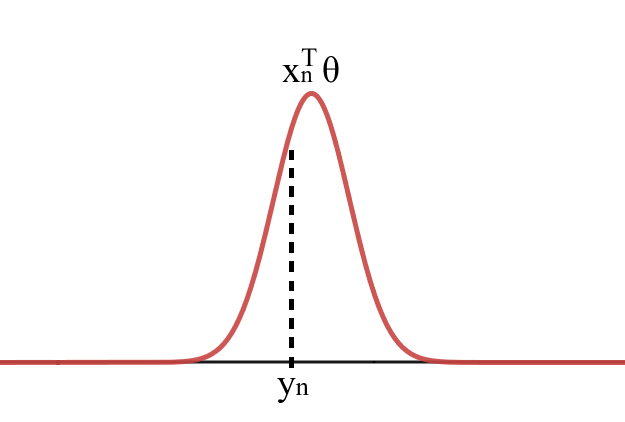
\includegraphics[width=.75\linewidth]{img/gaussian_mle_good.png}
                \caption{When the parameters are good, the label will be near the mean (i.e. predictor)}
            \end{subfigure}
            \hspace*{1em}
            \begin{subfigure}{.45\textwidth}
                \centering
                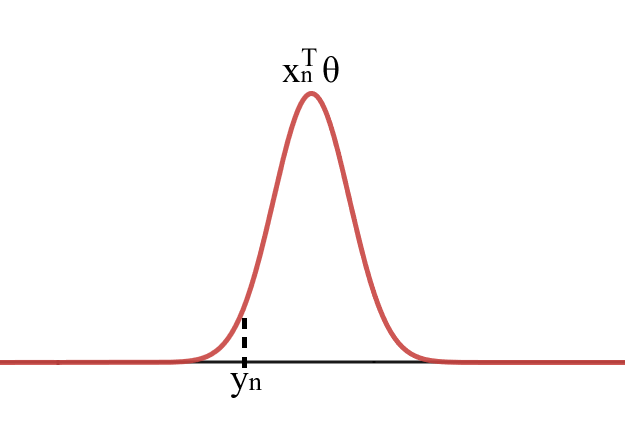
\includegraphics[width=.75\linewidth]{img/gaussian_mle_bad.png}
                \caption{When the parameters are bad, the label will be far from the mean}
            \end{subfigure}

            \caption{Geometric interpretation of the Gaussian likelihood}
        \end{figure}
\end{description}


\subsection{Maximum a posteriori estimation (MAP)}
\marginnote{Maximum a posteriori (MAP)}
Maximum a posteriori estimation uses the opposite distribution of MLE and maximizes:
\[ 
    \max_{\vec{\uptheta} \in \mathbb{R}^D} p(\vec{\uptheta} \vert \matr{X}, \vec{y}) =
    \min_{\vec{\uptheta} \in \mathbb{R}^D} -p(\vec{\uptheta} \vert \matr{X}, \vec{y})
\]
In other words, it maximizes the probability of a set of parameters $\vec{\uptheta}$ given the observation of the dataset $(\matr{X}, \vec{y})$.
By applying the Bayes' theorem, the problem becomes:
\[ 
    \begin{split}
        \min_{\vec{\uptheta} \in \mathbb{R}^D} 
            -\frac{p(\vec{y} \vert \matr{X}, \vec{\uptheta}) p(\vec{\uptheta})}{\underbrace{p(\vec{y} \vert \matr{X})}_{\mathclap{\text{constant}}}} &=
        \min_{\vec{\uptheta} \in \mathbb{R}^D} -p(\vec{y} \vert \matr{X}, \vec{\uptheta}) p(\vec{\uptheta}) \\
        &= \min_{\vec{\uptheta} \in \mathbb{R}^D} \{ -\log p(\vec{y} \vert \matr{X}, \vec{\uptheta}) -\log p(\vec{\uptheta}) \}
    \end{split}
\]

\begin{description}
    \item[Gaussian posteriori] \marginnote{Gaussian posteriori}
        By assuming that the conditional probability of the dataset follows a Gaussian distribution (as in MLE),
        the problem becomes:
        \[ 
            \min_{\vec{\uptheta} \in \mathbb{R}^D} \{ -\log p(\vec{y} \vert \matr{X}, \vec{\uptheta}) -\log p(\vec{\uptheta}) \} = 
            \min_{\vec{\uptheta} \in \mathbb{R}^D} \{ \Vert \vec{y} - \matr{\uptheta}\matr{X} \Vert^2 -\log p(\vec{\uptheta}) \} 
        \]

        Moreover, assuming that $p(\vec{\uptheta}) \sim \mathcal{N}(0, \matr{\Sigma})$, we have that:
        \[ -\log p(\vec{\uptheta}) = \frac{1}{2\sigma^2} \Vert \vec{\uptheta} \Vert^2 \]

        Therefore, the problem becomes:
        \[ \min_{\vec{\uptheta} \in \mathbb{R}^D} \{ \Vert \vec{y} - \matr{\uptheta}\matr{X} \Vert^2 + \lambda \Vert \vec{\uptheta} \Vert^2 \} \]
        MAP can be seen as a regularization factor for MLE.
\end{description}



\section{Linear regression}
\marginnote{Linear regression}
Given a dataset of inputs $\vec{x}_n \in \mathbb{R}^D$ with corresponding labels $y_n = f(\vec{x}_n) + \varepsilon$,
where $f: \mathbb{R}^D \rightarrow \mathbb{R}$ and $\varepsilon \sim \mathcal{N}(0, \sigma^2)$ is a Gaussian noise,
we want to estimate the function $f$.

\begin{description}
    \item[Model]
        We use as the predictor:
        \[ f(\vec{x}) = \vec{x}^T \vec{\uptheta} \]
        Because of the noise, we use a probabilistic model with likelihood:
        \[ p_\vec{\uptheta}(y \,\vert\, \vec{x}) = \mathcal{N}(y \,\vert\, f(\vec{x}), \sigma^2) \]

    \item[Parameter estimation]  
        To estimate $\vec{\uptheta}$, we can use MLE:
        \[ \min_{\vec{\uptheta} \in \mathbb{R}^D} -p_\vec{\uptheta}(\vec{y} \vert \matr{X}) \]
\end{description}


\subsection{Maximum likelihood estimation with features}
\marginnote{MLE with features}
Linear regression is linear only with respect to the parameters $\vec{\uptheta}$. 
Therefore, it is possible to apply any transformation to the inputs of the predictor $f$ such that:
\[ f(\vec{x}_n) = (\phi(\vec{x}_n))^T \vec{\uptheta}  \]
where $\phi: \mathbb{R}^D \rightarrow \mathbb{R}^K$ is a transformation and 
$\vec{\uptheta} \in \mathbb{R}^K$ are the parameters.

Given a dataset of $N$ entries $\vec{x}_n \in \mathbb{R}^D$ with labels $y_n \in \mathbb{R}$
and a transformation function $\phi: \mathbb{R}^D \rightarrow \mathbb{R}^K$,
the transformed features can be expressed through a feature matrix $\matr{\Phi} \in \mathbb{R}^{N \times K}$:
\[
    \matr{\Phi} = 
    \begin{pmatrix}
        (\phi(\vec{x}_1))^T \\ \vdots \\ (\phi(\vec{x}_N))^T
    \end{pmatrix} 
    =
    \begin{pmatrix}
        \phi_0(\vec{x}_1) & \cdots & \phi_{K-1}(\vec{x}_1) \\ 
        \vdots & \ddots & \vdots \\ 
        \phi_0(\vec{x}_N) & \cdots & \phi_{K-1}(\vec{x}_N) \\ 
    \end{pmatrix}
\]

The negative log-likelihood can be defined as:
\[ 
    -\log p_\vec{\uptheta}(\vec{y} \,\vert\, \matr{X}) =
    \frac{1}{2\sigma^2} (\vec{y} - \matr{\Phi}\vec{\uptheta})^T (\vec{y} - \matr{\Phi}\vec{\uptheta}) + \text{constant}
\]
As $\matr{\Phi}$ is (usually) full-rank and convex, the problem can be solved directly using normal equations:
\[ 
    \matr{\Phi}^T \matr{\Phi} \vec{\uptheta} = \matr{\Phi}^T \vec{y} \iff 
    \vec{\uptheta} = (\matr{\Phi}^T \matr{\Phi})^{-1} \matr{\Phi}^T \vec{y}
\]
Obviously, the negative log-likelihood can also be minimized by using a gradient method.

\begin{description}
    \item[Root mean square error (RMSE)] \marginnote{Root mean square error (RMSE)}
        RMSE is computed as:
            \[ 
                \sqrt{ \frac{1}{N} \Vert \vec{y} - \matr{\Phi}\vec{\uptheta} \Vert^2 } =
                \sqrt{ \frac{1}{N} \sum_{n=1}^{N}(y_n - (\phi(\vec{x}_n))^T\vec{\uptheta})^2 }
            \]
            Differently from MSE, RMSE allows to compare errors of datasets with different sizes
            and scales its result to the labels.

            By comparing the RMSE of the train and test sets, it is possible to check if a model is overfitting.
\end{description}

\begin{description}
    \item[Polynomial regression] \marginnote{Polynomial regression}
        The transformation function $\phi: \mathbb{R} \rightarrow \mathbb{R}^K$ is defined as:
        \[  
            \phi(x) = 
            \begin{pmatrix}
                \phi_0(x) \\ \phi_1(x) \\ \phi_2(x) \\ \vdots \\ \phi_{K-1}(x)
            \end{pmatrix}
            = 
            \begin{pmatrix}
                1 \\ x \\ x^2 \\ \vdots \\ x^{K-1}
            \end{pmatrix}
        \]
        The predictor is then defined as:
        \[ 
            \begin{split}
                f(x) &= (\phi(x))^T \vec{\uptheta} \\
                    &= \sum_{i=0}^{K-1} \phi_i(x)\vartheta_i = \sum_{i=0}^{K-1} x^i \vartheta_i
            \end{split}
        \]
\end{description}